\documentclass{article}
\usepackage{tikz}
\usepackage[a4paper]{geometry}
\usepackage{fancyhdr}
\pagestyle{fancy}
\lhead{Das subjektive Verfahren}
\rhead{April 2026}
\begin{document}
\section{Das subjektive Verfahren}
Anstelle der objektiven Messung zur Messung des Interferenzmusters eines Einzel- oder Doppelspalts oder dem Gitter kann auch das subjektive Verfahren genutzt werden.
 
Hier wird direkt auf das Gitter geschaut. Der Schirm ist die Netzhaut des Auges. Das Gehirn geht aber davon aus, dass alle Lichtstrahlen parallel seien, weshalb wir das Licht anderswo wahrnehmen.
\begin{center} 
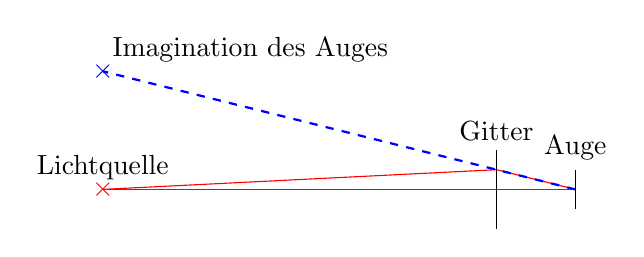
\begin{tikzpicture} 
 \draw[red] (0, 0) -- (6, 0);  
 \draw[red] (5, 0) -- (5, 0);
 \draw[red] (0, 0) -- (5, 0.25);
 \draw[red] (5, 0.25) -- (6, 0);
 \draw[blue, dashed, thick] (6, 0) -- (0, 1.5); 
 
 \node[red] at (0, 0) {$\times$} node[above, black] {Lichtquelle};
 \draw (5, -0.5) -- (5, 0.5) node[above] {Gitter};
 \draw (6, -.25) -- (6, .25) node[above] {Auge};  
 \node[blue] at (0, 1.5) {$\times$};
 \node[above right] at (0, 1.5) {Imagination des Auges};
\end{tikzpicture}
\end{center}
Wird über die Lichtquelle ein Lineal platziert, so kann die Distanz zwischen dem Maximum nullter Ordnung und dem Ort, an dem das Gehirn das Licht meint zu sehen, bestimmt werden.
\end{document}